% !TeX spellcheck = cs_CZ
%{\tikzset{external/prefix={tikz/CES/}}
% \tikzset{external/figure name/.add={ch05_}{}}
%---------------------------------------------------------------------------------------------------
% file ANSI_C_MCU.tex
%---------------------------------------------------------------------------------------------------
%============================= Kapitola: Stručný úvod===============================================
\setchaptertoc
\chapter{Programování vestavěných systémů}\label{ces:C_chapI}

  Tato kapitola demonstruje programování vestavěných systémů s využitím různých nástrojů s 
  otevřeným zdrojovým kódem, včetně sady \wikiGCC (GCC), což je standardní sada překladačů 
  vytvořených v rámci projektu GNU, který je v tomto oboru běžně používán. 
  
%  Each embedded system is unique, and the hardware is highly specialized to the application 
%  domain. As a result, embedded systems programming can be a widely varying experience and can 
%  take years to master. However, one common denominator across almost all embedded software 
%  development is the use of the C programming language. This book will teach you how to use C in 
%  any embedded system.
  
  Každý vestavěný systém je unikátní, což souvisí s tím, že hardware je silně specializovaný pro 
  danou aplikaci. Z toho vyplývá, že programování těchto systémů vyžaduje velké zkušenosti, neboť 
  programátor není odstíněn od hardware. Pokud se zeptáme, co mají tyto systémy společného, pak 
  jednoznačnou odpovědí je, že se programují jazykem \texttt{C}.
  
  V současné době je to jeden z nejpopulárnějších jazyků a to nejen pro aplikace v zabudovaných 
  systémech (viz \ref{chap:ces_arm}), ale zřejmě také je nejčastějším jazykem pro psaní systémového 
  softwaru.
  
  %============= Podkapitola: Základní pojmy =======================================================
  \section{Stručná historie a charakteristika jazyka  C}\label{ces:C_chapIsecI}
     Pro programátory, kteří pracují s jinymi jazyky, může byt užitečné pro srovnání se dozvědět o 
     historických, technických a filozofickych aspektech jazyka \texttt{C}. 
     
    \wikiANSIC vznikl počátkem 70. let 20. století. Jazyk vyvinuli \emph{Ken Thompson} a 
    \emph{Dennis Ritchie} (obr. \ref{ces:fig037}) pro potřeby operačního systému \texttt{Unix}.  
    
    \texttt{C} lze charakterizovat je nízkoúrovňový, kompilovaný, relativně minimalistický 
    programovací jazyk. Je také dostatečně mocný na většinu systémového programování (ovladače a 
    jádro OS), přičemž zbytek lze dořešit tzv. \wikiInlineASM, tedy metodou zápisu assembleru přímo 
    do kódu. Zdrojový kód \texttt{C} je přitom mnohem čitelnější než assembler, je jednodušší ho 
    zapsat a navíc je daleko snáze přenositelný na jiné procesory a počítačové architektury. Proto 
    jsou často operační systémy, překladače, knihovny a interprety vysokoúrovňových jazyků 
    implementovány právě v \texttt{C}. 
    
    Mnoho dalších moderních programovacích jazyků přebírá způsob zápisu (neboli syntaxi) z jazyka 
    \texttt{C}, například \wikiCPP, Java, Perl a PHP.

    \luagraphic[1]{ces_fig037.jpg}{Autoři jazyka \texttt{C} Ken Thompson a Dennis Ritchie přebírají
    ocenění v podobě Národní medaile za technologii (v roce 1998) od Billa Clintona}{ces:fig037} 
    
    V roce 1973 se stal jazyk \texttt{C} dostatečně stabilním. Proto většina zdrojového kódu jádra 
    \texttt{Unixu}, původně napsaného v assembleru, byla přepsána do \texttt{C}. \texttt{Unix} tedy 
    patří mezi první operační systémy, které byly napsané v jiném než strojovém jazyce či 
    assembleru. To také přispělo k velké popularitě tohoho jazyka. 
    
    V roce 1978, Ritchie a Brian Kernighan vydali famózní knihu \emph{The C Programming Language}. 
    Tato kniha, mezi programátory \texttt{C} známá jako „K\&R“, sloužila po mnoho let jako 
    neformální specifikace jazyka. Verze C, kterou takto popsali, bývá označována jako 
    „\textbf{K\&R C}\footnote{Druhé vydání knihy popisovalo novější standard \texttt{ANSI C}.}“.
                        
    Dalšími milníky vývoje jazyka \texttt{C} jsou dány standardizačnímy procesy organizace American 
    National Standards Institute (ANSI) a International Organization for Standardization ISO:
    \begin{description}
      \item[C89]    V roce 1983 se \texttt{ANSI} dohodla na sestavení komise, aby vytvořila 
                    standardní specifikaci C. Po dlouhém procesu byl standard dokončen v roce 1989 
                    a schválen jako ANSI X3.159-1989 „\emph{Programming Language C}“. Tato verze 
                    jazyka je často stále označována jako \textbf{ANSI C} nebo \textbf{C89}.
      \item[C90]    V roce 1990 byl standard ANSI C (s drobnými změnami) adoptován institucí ISO 
                    jako „ISO 9899-ISO/IEC 9899:1990“. Formálně tak nahradil předchozí verzi 
                    C89/ANSI-C a tato revize je označována jako \textbf{C90} neboli \uv{jazyk C}. 
                    Technicky je to stejný standard jako C89/ANSI-C.
      \item[C99]    Po standardizaci jazyka v roce 1989 - 1990 se většina vývoje soustředila na 
                    jazyk \texttt{C++}. Přesto však na konci 90. let došlo k vydání dokumentu ISO 
                    9899:1999 (obvykle nazývaný \textbf{C99}), který byl následně v březnu 2000 
                    přijat i jako ANSI standard. C99 představil několik nových vlastností, které 
                    byly mnohdy v překladačích už dávno implementovány jako rozšíření.
      \item[C11]    V roce 2007 začala práce na další revizi standardu \texttt{C}, neformálně 
                    nazývaného "C1X", až do oficiálního zveřejnění dne 2011-12-08. Výbor pro 
                    standardy \texttt{C} přijal pokyny, které omezují přijetí nových funkcí, které 
                    nebyly testovány stávajícími implementacemi.
    \end{description}
    
    \begin{tcnote}
      První norma pro \texttt{C} byla tedy vydána společností ANSI. Ačkoli tento dokument byl 
      následně přijat Mezinárodní organizací pro normalizaci (ISO) a následné revize vydané 
      společností ISO byly také přijaty ANSI, mnozí programátoři stále používají "\emph{ANSI C}", 
      ačkoliv se odkazují na ISO standard. Jiní vývojáři softwaru používají termín \emph{ISO C}, 
      ostatní jsou neutrální a používají \emph{Standard C}.
    \end{tcnote}
  
  %============= Podkapitola: Základní pojmy =======================================================
  \section{Konstrukce a struktura programu v jazyce C}\label{ces:C_chapIsecII}
    Konstrukce programu \texttt{C} je velmi jednoduchá, neboť program je strukturovaný do 
    přehledných bloků. Základní blok, jemuž jsou všechny ostatní
    bloky podřízeny, je funkční blok, jednodušeji označovaný jako „\emph{funkce}". Celý program
    se pak skládá z množiny funkcí, které obsahují a zpracovávají data a proměnné a jejich 
    prostřednictvím vzájemně komunikují.
    
    Použití funkcí není nic nového a provádí se i v jiných programovacích jazycích prostřednictvím 
    podprogramů, procedur apod.
    
    U mikrokontrolérů se před vyvoláním programu \texttt{C} spouští počáteční (\emph{startup})
    modul, programový modul napsaný většinou v assembleru. Jeho prostřednictvím se provádí základní 
    inicializace různých registrů mikrokontroléru, oblastí paměti, ukazatelů zásobníku (\emph{stack 
    pointer}) a vektorů přerušení. Po tomto spouštěcím kódu začíná i pro mikrokontrolér běh 
    programu \texttt{C} vždy funkcí s názvem \textbf{main()}, která je vyvolána startup modulem. 
    Proto je založení této funkce povinné. Po spuštění programu převezme funkce main() řízení, 
    zpracovává postupně příkazy a podle naprogramovaného zdrojového kódu C volá další funkce. V 
    kap. \ref{ces:C_chapIsecIV} budou vlastnosti, zakládání a volání \texttt{C} funkcí popsány 
    podrobněji. Na tomto místě uvedeme jen základy, abychom mohli založit první funkci main.

    
    \subsection{Způsob zpracování C programu}
      Chceme-li jazyk C opravdu využívat, je nutné seznámit se trochu více s tím, jak se program 
      vlastné zpracovává, od napsání zdrojového text až po spuštění přeloženého a sestaveného 
      programu.
      
      Základní zpracování programu v \texttt{C} probíhá několika fázemi schematicky vyjádřenými 
      následujícím obrázkem: 

      \luagraphic[1]{ces_fig008.png}{Zpracování zdrojového textu do podoby spustitelného programu 
      \texttt{EXE}}{ces:fig008}
      
      Jednotlivé programy, kterými je zdrojový soubor zpracován mají tento význam:
      \begin{description}
        \item[Editor] Pomocí něj se vytváří a opravuje zdrojový (\texttt{.C}) soubor. Při výběru se 
          uplatňuje tolik vlivů, že prakticky o žádném editoru nelze tvrdit, že je nejlepší či 
          horší. Pokročilé editory, nabízí možnost přizpůsobitelné syntaxe a zvýraznění klíčových 
          slov, vyhledávání a nahrazování, HEX režim, atd.
        \item[Preprocesor] je součást překladače, která předzpracovává (upravuje) zdrojový soubor 
          tak, aby měl překladač snadnější práci. Např. vynechává komentáře, zajišťuje správné 
          vložení hlavičkových (\texttt{.H}) souborů, rozvoj maker, atd. Výsledkem jeho práce je 
          opět textový soubor.
        \item[Compiler] Nazývaný též \emph{překladač} nebo počeštěně \uv{kompilátor}, provádí      
          překlad zdrojového souboru (zpracovaného již preprocesorem) do relativního (objektového) 
          kódu mikrokontroléru - vzniká \texttt{.OBJ} nebo \texttt{.O} soubor. Relativní 
          kód\footnote{Který se oficiálně nazývá jazyk relativních adres} je téměř hotový program. 
          Slovo relativní znamená, že adresy proměnných nebo funkcí ještě nejsou vůbec známy (např. 
          proto, že jsou uloženy v knihovně) a jsou tedy v \texttt{.OBJ} souboru zapsány relativně. 
          Vedlejším produktem překladače je tzv. protokol o překladu (\texttt{.LIS}), ve kterém je 
          uložena informace o chybách nalezených překladačem. 
        \item[Linker] Neboli \emph{sestavovací program} přidělí relativnímu kódu (respektive jeho 
          relativním adresám) absolutní adresy a převede všechny odkazy (najde adresy) na dosud 
          neznámé identifikátory (např. na volané knihovní funkce uložené v souborech 
          \texttt{.LIB}). Výsledkem práce linkeru je přímo spustitelný program (\texttt{.EXE}). 
        \item[Debugger] Český překlad je "odvšivovač", se neujal. Spíše se používá pojem 
          \emph{ladící program}. Slouží pro ladění, neboli odhalování chyb, které nastávají při 
          běhu programu. Po nalezení chyby se celý cyklus (editor, compiler, linker, debugger) 
          opakuje tak dlouho, až si myslíme, že náš program žádnou chybu neobsahuje. 
      \end{description}
      
    \subsection{Základní typy: int, char, float, double}
    \subsection{Velikost datového typu int}
      Programátoři se ne vždy starají o to, jaké paměťové nároky má datový typ \textbf{int}. 
      Prohlédněme si následující příklad:
      \begin{lstlisting}[style=luaCStyle]
        int i;         
        for (i = 0; i < N; i++) { ... } 
      \end{lstlisting}
      Obecně očekáváme, že překladač (\emph{compilator}) vygeneruje co nejefektivnější kód, a 
      zároveň předpokládáme, že během inkrementace proměnné \texttt{i} smyčkou 
      \lstinline[style=luaCStyle]!for! nevznikne číslo, které by nešlo uložit do překladačem 
      zvoleného místa v paměťi, které může mít velikosti 8, 16, 32 nebo třeba 64 bitů. A to je 
      přesně to, co standardy \texttt{ISO C} a  \texttt{C++} říkají tvůrcům překladače: vybrat 
      nejefektivnější velikost datového typu, která splní konkrétní požadavek. Velikosti celých 
      čísel u různých typů procesorů není pevná. Spolu s odpovídající flexibilitou standardů jazyka 
      \texttt{C}, bude v předchozím kódu proměnná \texttt{i} chápana jako 32bitové nebo 16bitové 
      celé číslo v závislosti na použitém překladači a to i v případě, že cílový (\emph{target}) 
      mikrokontrolér je stejný. Lze snadno pochopit, že závislost velikosti proměnné datového typu 
      int na zvoleném mikrokontroléru a použitém překladači je pro přenosné programy v \texttt{C} 
      velmi nevýhodná(\cite[s.~29]{Barr2009}).
      
      Na velikosti datového typu \texttt{int} (např. \textbf{Embedded programming}) tedy z mnoda 
      důvodů záleží. Tuto problematiku vyřešil až standard \texttt{C99}, který závádí v hlavičkovém 
      souboru (header file) \wikiSTDINT například tyto nové datové typy int: 
      \begin{itemize}[noitemsep]
        \item  8-bitů: \textbf{int8\_t},  \textbf{uint8\_t}
        \item 16-bitů: \textbf{int16\_t}, \textbf{uint16\_t}
        \item 32-bitů: \textbf{int32\_t}, \textbf{uint32\_t}
      \end{itemize}


  %============= Podkapitola: Konstrukce a struktura programu v jazyce C ===========================

  %============= Podkapitola: Proměnné datové typy, rozsahy platnosti a hodnot =====================
  \section{Proměnné datové typy, rozsahy platnosti a hodnot}\label{ces:C_chapIsecIII}
  %============= Podkapitola: Operátory ============================================================
  \section{Operátory}\label{ces:C_chapIsecIV}
    \subsection{Bitové  operátory}
      Protože jazyk \texttt{C} je oproti jiným vyšším jazykům zaměřen na přeci jen poněkud nižší 
      úroveň, 
      nabízí programátorům i operátory, pomocí kterých mohou nepřímo pracovat i s jednotlivými bity.
      Tuto možnost zdaleka nemají všechny programovací jazyky označované jako \emph{vyšší}.
      
      Bitové operátory \(<<\), \(>>\), \&, \(\lvert\), \~, \^, tedy posun vlevo, posun vpravo, and,
      or, not a xor jsou povoleny pouze pro celočíselné (integer) datové typy char, int, short, long
      (se znaménkem (signed) nebo bez znaménka (unsigned)). V závislosti na MCU a kompilátoru se
      tyto příkazy převádějí na odpovídající výkonné strojové instrukce. Toto hardwarově blízké
      bitové řízení často nalézá uplatnění při přístupu na speciální registry v mikrokontroléru.
      (\cite[s.~79]{Burkhard2003}).
      
      Při bitovém posunu vlevo (vpravo) << , ( >> ) se jednotlivé bity posouvají vlevo (vpravo), 
      tedy do pozice s (binárně) vyšším (nižším) řádem. Na nejpravější (nejlevější) posunem 
      vytvořenou pozici je umístěna nula. Posuny ovšem probíhají aritmeticky. To znamená, že 
      uvedené pravidlo neplatí pro posun vpravo hodnoty celočíselného typu se znaménkem. V takovém 
      případě se nejvyšší bit (znaménkový), zachovává. Takto se při posunu doplňuje do bitového 
      řetězce nový bit. Naopak před posunem nejlevější (nejpravější) bit je odeslán do
      "říše zapomnění.
      
      Bitový posun o jeden (binární) řád vpravo, respektive vlevo, má stejný význam, jako 
      celočíselné dělení, respektive násobení, dvěma. Je-li bitový posun o více než jeden řád, 
      jedná se o násobení (dělění) příslušnou mocninou dvou.
      
      Bitové and \& , or \(\lvert\), a xor \^ provádí příslušnou binární operaci s každým párem 
      odpovídajících si bitů. Výsledek je umístěn do pozice stejného binárního řádu výsledku. 
      Výsledky operací nad jednotlivými bity jsou  stejné, jako v Booleově algebře. Bitové not \~ 
      je operátorem unárním, provádí negaci každého bitu v bitovém řetězci jediného operandu. 
      Tomuto operátoru se často říká bitový doplněk. 
      
      \subsubsection{Makra pro bitové operace}
        O něco elegantnější je použití maker k nahazování, shazování a testování bitových míst. 
        \begin{lstlisting}[gobble=10, xrightmargin=13em]
          #define SET_BIT(REG, BIT)     ((REG) |= (BIT))
          #define CLEAR_BIT(REG, BIT)   ((REG) &= ~(BIT))
          #define READ_BIT(REG, BIT)    ((REG) & (BIT))
        \end{lstlisting}
       Takto vypadají makra pro bitové operace: nastav bit, smaž bit, čti bit v knihovně 
       \texttt{STM32F4 Library} (\texttt{stm32f4xx.h})
      
  %============= Podkapitola: Pointery =============================================================
  \section{Pointery}
    \textbf{Pointery} (též ukazatele nebo směrníky) jsou \emph{"srdce a duše jazyka C"}. Pointer je 
    proměnná, jako každá jiná, pouze hodnota uložená v této proměnné má jiný význam. Pointer 
    představuje \textit{adresu paměti} a na této adrese se teprve ukrývá příslušná hodnota. Pointer 
    je tedy proměnná uchovávající paměťovou adresu.\cite{Herout}
  
    \subsection{Práce s pointery}
      \begin{figure}
        \centering
        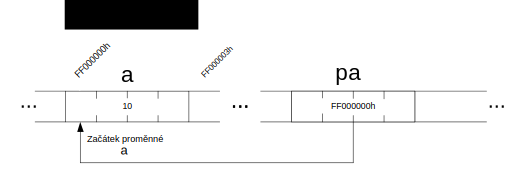
\includegraphics[width=0.9\linewidth]{princip_ukazatele.pdf}
        \caption{Princip ukazatele v paměti}
        \label{figure:pointer1}
      \end{figure}

      %--funkce kopírující prvky jednoho pole do druhého--------------
        % !TeX spellcheck = cs_CZ
\begin{mdframed}[style=mdexam]
  \begin{example}Vytvořte funkce kopírující prvky jednoho pole do druhého pomocí indexu i 
    ukazatele.      
    %---------------------------------------------------------------
    \lstinputlisting[style=luaCStyle, firstline=8, 
      caption=\texttt{CPYARRY.C} Kopíruje prvky jednoho pole do 
      druhého.]{../src/CES/C/CPYARRY.c}
    %---------------------------------------------------------------    
    Výstup programu:%
    \begin{mdframed}[style=mdmsdos]
      \texttt{\textbf{1   2   3   4   5   6   7   8   9}} \\
      \texttt{\textbf{1   2   3   4   5   6}} \\
      \texttt{\textbf{4   5   6   7   8   9}}
    \end{mdframed}
  \end{example}
\end{mdframed}
      %---------------------------------------------------------------
  %============= Podkapitola: Preprocesor jazyka C =================================================
  \section{Preprocesor jazyka C}
    Preprocesor interpretuje jednoduché direktivy pro vložení zdrojového kódu z jiného souboru 
    (\lstinline[style=luaCStyle]!#include!), definice maker 
    (\lstinline[style=luaCStyle]!#define!) a podmíněné vložení kódu 
    (\lstinline[style=luaCStyle]!#if!). \texttt{C} preprocesor přijímá tyto direktivy:
    
    \begin{table}[ht!]
      \centering
      \begin{tabular}{c c c c}
        \hline
        \lstinline[style=luaCStyle]!#define!  & \lstinline[style=luaCStyle]!#elif! & 
        \lstinline[style=luaCStyle]!#else!    & \lstinline[style=luaCStyle]!#endif!  \\
        \lstinline[style=luaCStyle]!#error!   & \lstinline[style=luaCStyle]!#if! & 
        \lstinline[style=luaCStyle]!#ifdef!   & \lstinline[style=luaCStyle]!#ifndef! \\
        \lstinline[style=luaCStyle]!#include! & \lstinline[style=luaCStyle]!#line! & 
        \lstinline[style=luaCStyle]!#pragma!  & \lstinline[style=luaCStyle]!#undef!  \\
        \hline            
      \end{tabular}
      \caption{Seznam platných direktiv jazyka \texttt{C}}\label{S4101C1:C_tab_direktiva}
    \end{table} 
    
    \subsection{Připojení externích souborů}
    
    \subsection{Definice maker}
      Definice maker ve významu rozsahů polí je typickým příkladem použití preprocesoru. Ve 
      zdrojovém textu se neodvoláváme na magická čísla, ale na vhodně symbolicky pojmenovaná makra, 
      která zvýší čitelnost programu.
      
      Pro větší přehlednost rozdělme makra na 
      \begin{itemize}
       \item symbolické konstanty,
       \item makra
      \end{itemize}
      Klíčem nechť je skutečnost, že makro na rozdíl od symbolické konstanty má argumenty.
      \subsection{Symbolické konstanty}
      \subsection{Makra}
     
    \subsection{Podmíněný překlad}  
      Preprocesor může během své činnosti vyhodnocovat, je-li nějaké makro definováno, či nikoliv. 
      Při použití klíčového slova preprocesoru \texttt{defined} pak může spojovat taková 
      vyhodnocení do rozsáhlejších logických výrazů. Argument defined nemusí být uzavřen do 
      závorek. Může se však vyskytnout jen za \lstinline[style=luaCStyle]!#if! nebo 
      \lstinline[style=luaCStyle]!#elif!. Například si ukažme složitější podmínku:


  %============= Podkapitola: Terminálový vstup a výstup============================================
  \section{Terminálový vstup a výstup}
    Jazyk C, narozdíl od Pascalu, nedefinuje žádnou \texttt{I/O (vstup\-ně/výstup\-ní 
    -In\-put/Out\-put)} operaci jako část jazyka. Nezbytné vstupy a výstupy jsou řešeny tak, že 
    standardní knihovna obsahuje několik funkcí, které \texttt{I/O} zajišťují.
  
    Nejvíce strojově závislé akce jsou I/O operace a tímto způsobem se tedy důsledně oddělují 
    strojově závislé a strojově nezávislé části jazyka. Tato skutečnost je pak významným přínosem 
    při vytváření kompilátoru pro jiný počítač.
  
    \begin{figure}[ht!]
      \centering
      
\includegraphics[scale=1.2]{terminalovy_IO_skica.pdf}
      \caption{Operace pro terminálový vstup a výstup}\label{C:fig_Terminal_IO}
    \end{figure}
  
    \subsection{Hlavičkový soubor \texttt{stdio.h}}
      Aby bylo možno správně používat všechny funkce pro vstupu a výstupu, je nutné na začátku 
      programu připojit "popis" těchto funkcí. Ten se nachází v hlavičkovém (\emph{header}) souboru 
      \lstinline[style=luaCStyle]!stdio.h!:
  
      \lstinline[style=luaCStyle]!#include <stdio.h>  //zde neni strednik!
  
      Od tohoto okamžiku je pak možné používat dále popsané funkce.
  
    \subsection{Standardní vstup a výstup znaku}
      Výstup jednoho znaku zajišťuje \lstinline[style=luaCStyle]!putchar()! a vstup jednoho 
      znaku funkce \lstinline[style=luaCStyle]!getchar()!.
      \begin{itemize}
        \item \lstinline[style=luaCStyle]!int putchar(int c);!
        \item \lstinline[style=luaCStyle]!int getchar(void);!
      \end{itemize}
      Obě funkce pracují s proměnnými \lstinline[style=luaCStyle]!int! a ne 
      \lstinline[style=luaCStyle]!char!.
  
        % \marginpar{\includegraphics[width=0.09\textwidth]{pen.pdf}}
        %---------------------------------------------------------------
        \lstinputlisting[style=luaCStyle, caption=\texttt{Cteni\_tisk\_znaku.c} Čtení a tisk znak ze  
          standardního vstupu na standardní výstup.]{../src/CES/C/Cteni_tisk_znaku.c} 
        %--------------------------------------------------------------    
      
      \begin{example}Čtení znaku ze standardního vstupu a jejich zápis na standardní výstup 
        ukazuje následující program, představující jednoduchou variantu příkazu kopírování souboru 
        (nutno ovšem přesměrovat vstup a výstup).
  
        % \marginpar{\includegraphics[width=0.09\textwidth]{pen.pdf}}
        %---------------------------------------------------------------
        \lstinputlisting[style=luaCStyle, caption={\texttt{CPY.c} Kopíruje znak ze standardního
          vstupu na standardní výstup.}]{../src/CES/C/CPY.c}
        %---------------------------------------------------------------
      \end{example}
      
    \subsection{Standardní vstup a výstup řetězců}
      Standardní vstup a výstup řetězců je jednoduchou nadstavbou nad čtením znaku. Obě funkce,
      \begin{itemize}
        \item \lstinline[style=luaCStyle]!char *gets(char *s);!
        \item \lstinline[style=luaCStyle]!int puts(const char *s);!
      \end{itemize}
      pracují s řetězci. \texttt{gets()} načte do znakového pole vstupní řetězec az do konce řádku, 
      symbol  \lstinline[style=luaCStyle]!'\n'! není do znakového pole zapsán. Ukazatel na 
      pole (načtený řetězec) je rovněž návratovou hodnotou. Chybu signalizuje návrat NULL. 
      \texttt{puts()} 
      zapíše řetězec na výstup a přidá přechod na novy řádek       
      \lstinline[style=luaCStyle]!'\n'!. Chybu představuje návratové \texttt{EOF}, jinak vrací 
      kladné cele číslo.
  
      Jednoduchost použití skrývá velké nebezpečí. Funkce \texttt{gets()} nemá informaci o délce 
      oblasti vymezené pro čtený řetězec. Je-li oblast kratší, než vstupní řádek, dojde jeho 
      načtením velmi pravděpodobně k přepsání paměťové oblasti související s vyhrazenou pamětí. A 
      to se všemi důsledky z toho vyplývajícími.
  
    \subsection{Formátovaný standardní vstup a vystup}
    \subsection{Souhrnné cvičení}
      \begin{example}Vytvořte program, který vygeneruje ASCII tabulku se čtyřmi sloupci ve formátu
      \textbf{[znak\(\lvert\)kód\(\lvert\)znak\(\lvert\)kód]}. Rozsah tabulky definujte pomocí dvou
      symbolických konstant \lstinline[style=luaCStyle]!MIN_ASCII, MAX_ASCII!. 
  
        % \marginpar{\includegraphics[width=0.09\textwidth]{pen.pdf}}
        %---------------------------------------------------------------
        \lstinputlisting[style=luaCStyle, caption=\texttt{ASCII.c} Generuje ASCII tabulku na 
          terminálu.]{../src/CES/C/ASCII.c}
        %---------------------------------------------------------------
      \end{example} 

%} % tikzset
%---------------------------------------------------------------------------------------------------